\documentclass[licencjacka,en]{pracamgr}
\usepackage{dirtytalk}
\usepackage{hyperref}
\usepackage{graphicx}
\usepackage{cellspace}
\setlength\cellspacetoplimit{5pt}
\setlength\cellspacebottomlimit{5pt}
\graphicspath{ {./images/} }

\autor{Tomasz Nowak}{429575}
\autori{Michał Staniewski}{429598}
\autorii{Mieszko Grodzicki}{429132}
\autoriii{Bartosz Smolarczyk}{429594}
\opiekun{mgr Michał Możdżonek\\
  Institute of Informatics\\
  }
\date{May 2023}
\kierunek{Computer Science}
% Wg klasyfikacji Socrates-Erasmus:
\dziedzina{
11.3 Computer Science\\
}
% Klasyfikacja tematyczna wedlug AMS (matematyka) lub ACM (informatyka)
\klasyfikacja{
  D. Software\\
  D.2. Software Engineering\\
  D.2.4. Software/Program Verification
  }

\title{Accelerating package expansion in Rust through development of a semantic versioning tool}
\titlepl{Przyspieszenie rozwoju pakietów w języku Rust poprzez rozbudowę narzędzia do
	semantycznego wersjonowania}
\keywords{Rust, semantic versioning, continuous integration, package manager}

\begin{document}
\maketitle

\begin{abstract}
In many programming languages there exist countless nuances, making developers accidentally release
new versions of their packages that are not backwards-compatible. Such releases can directly impact
projects which are using their packages, causing bugs or even compilation errors when using the
latest version. One of the affected languages is Rust, which also lacks (itself) a built-in
mechanism for enforcing semantic versioning.

The aim of this thesis is to describe the development of a tool for Rust programmers to reduce the
chances of publishing a new version of the code that violates semantic versioning.

There are already on-going plans to bundle this tool into the language's standard
development toolchain. It would make it commonly used and therefore help users to safely get
bug fixes, security patches and new functionality, without worrying about their app being broken
by a dependency change.
\end{abstract}

% Abstrakt po polsku (potrzebny tylko w APD?)
% W wielu językach programowania istnieją liczne niuanse sprawiające, że deweloperzy omyłkowo
% publikują nowe wersje swoich pakietów bez zachowania kompatybilności wstecznej. Takie sytuacje
% mogą bezpośrednio wpłynąć na projekty korzystające z ich pakietów, powodując błędy bądź nawet
% uniemożliwiając kompilację po aktualizacji do najnowszej wersji. Jednym z języków dotkniętych
% tym problemem jest Rust, który nie posiada wbudowanego mechanizmu wymuszającego
% semantyczne wersjonowanie.

% Celem tej pracy jest przedstawienie rozwoju narzędzia dla języka Rust, które zmniejsza ryzyko
% publikacji kodu nieprzestrzegającego zasad semantycznego wersjonowania.

% Są również plany, aby narzędzie to stało się częścią standardowego toolchainu deweloperskiego.
% Skutkowałoby to jego powszechnym użyciem i tym samym zagwarantowałoby użytkownikom, że korzystanie
% z poprawek błędów, łatek bezpieczeństwa oraz nowych funkcjonalności pakietów nie doprowadzi do
% awarii ich aplikacji.

\tableofcontents
%\listoffigures
%\listoftables

\chapter*{Executive summary}
\addcontentsline{toc}{chapter}{Executive summary}

TODO:
\begin{itemize}
	\item write the executive summary (around one page long)
	\item describe in short what is the goal of the project and what it solves
	\item describe that the project is indeed needed
	\item mention what we've done and how it moved the project towards the vision
	\item mention the results and the impact on the community
\end{itemize}

\chapter*{Introduction}
\addcontentsline{toc}{chapter}{Introduction}

Rust is a relatively new language that has lately been gaining on popularity. Amongst its standard
development toolchain there is a software called cargo -- Rust's build system and package manager,
which handles building a crate -- a package with Rust code. One of cargo's responsibilities is to
search for the newest crate versions, download them and build dependencies (that is, other
libraries / crates that the code uses).

Cargo assumes that all crates follow semantic versioning -- a set of rules that decide when it is
safe to use the new version of a library without any problems (the projects that depend on this
library must still compile). Thanks to that, developers of libraries can release patches and
bugfixes and cargo by default will automatically use those newest releases. The exact definition of
semantic versioning is explained in chapter \ref{r:chapter_definitions}.

It turns out that it is not obvious which changes are backwards-compatible and which are not.
There are numerous examples (listed in section \ref{r:section_rust_semver_problems})
where experienced Rust developers made a mistake (due to insufficient knowledge about the language
or by overlooking something) that changed the public API (Application Programming Interface)
of a library in such a way that users' code stopped compiling.

The authors of this thesis present their work on a tool that detects and notifies about a subset of
problems that make Rust libraries' public API non-backwards compatible, with the goal to make
problems with semantic versioning less frequent in the Rust community. The exact goals of this
project are described in chapter \ref{r:chapter_vision}.

The project is open-source -- all of the authors' work is visible in public repositories (listed in
\ref{r:section_projectstructure}). The project existed before their contributions, thus chapter
\ref{r:chapter_implementation} mainly describes how they have extended the project's
functionalities and fixed its issues. Chapter \ref{r:chapter_evaluation} is a summary of their
results and the project's impact on the Rust community.

%%%%%%%%%%%%%%%%%%%%%%%%%%%%%%%%%%%%%%%
%             Definitions             %
%%%%%%%%%%%%%%%%%%%%%%%%%%%%%%%%%%%%%%%

\chapter{Definitions}\label{r:chapter_definitions}

\section{Rust language}\label{r:section_rust_language}

With its first stable release in 2015, Rust is a relatively new programming language that
puts a strong emphasis on type-safety, memory-safety, performance and concurrency. Unlike
other memory-safe languages, Rust does not use reference counting nor a garbage collector.
Instead it tracks the object lifetime of all the program's references during compilation,
using its built-in mechanism named \say{borrow checker}.

Among many benefits and advantages of using Rust, there are three dominant features. Firstly,
it provides the user with a great performance, both time- and memory-wise, allowing for
writing efficient applications. Secondly, it is reliable -- with extensive type system and
focus on runtime safety, Rust prevents the user from making multiple bugs
already during compilation. Finally, it boosts productivity -- its documentation is
comprehensive and the compiler's error messages are clear and helpful. Rust also provides
an easy to use, integrated package manager and a dedicated build tool (named cargo),
an auto-formatter and many more.

According to surveys \cite{survey} conducted amongst developers, Rust is considered to be the most
enjoyable programming language for the 7th year in a row (as of 2022 summary, meaning it was always
on top since its release in 2015). Over 87\% of respondents who have previously used Rust would
like to continue programming in it.

Because of the high level of safety it provides, Rust has also become the secondary
language for writing the Linux kernel (with the primary being C). While there have been
attempts to add other languages (f.e. C++ in 1997), Rust is the first one to successfully
make it since the kernel's first release in 1991.

\section{Rust's package manager and build system -- cargo}\label{r:section_cargo}

Cargo is the official package manager for Rust. It is responsible for compiling the user's
packages, downloading their dependencies and uploading them to the selected package registry.
It is important to note that in Rust, packages are often refered to as \texttt{crates} with both
names being equivalent and commonly used. Most of the currently publicly available crates are
stored in the Rust community's default crate registry, \texttt{crates.io}. The role of the
registries is to allow users to easily find appropriate crates for their projects, as well as
publish their own work to be used by others. Each registry contains an index, which itself has
a searchable list of all the crates available within its registry. Cargo uses the selected registry
and index to download crates and update dependencies.

One can think of cargo as the Rust analogue of Python's pip (the recommended package manager for
Python). But despite their similar roles,
cargo has many advantages making it a lot safer than pip:
\begin{itemize}
	\item Cargo's crates are always installed using virtual environments, thus they cannot be
		installed in a location that would interfere with unrelated code.
	\item When a user adds a crate to their project, they can only use its direct, public interface.
		There is no possibility to access the interfaces of the dependencies that the added crate
		is using itself.
	\item The dependency's name must also be included in a special file named \texttt{Cargo.toml},
		not just in the source code file.
	\item To make the package's public interface explicit, Rust provides a series of tools for
		privacy management. Because of this, it is much more difficult for the user to make their
		project depend on something that the package's author did not intend to offer and could
		make private in future versions, causing a difficult to detect break on the user's end.
	\item Compatibility is taken seriously in Rust, thus packages' APIs (Applications Programming
		Interfaces) are expected to be backwards-compatible (and to follow semantic versioning,
		described in section \ref{r:section_semver}) when a new version is released. When a package
		does not satisfy this requirement, there exists a procedure called \textit{yanking}.
		It allows to remove the faulty version from the index without deleting any data, but moves
		the index back to the most recent working version. Yet in case an incompatible package is
		downloaded before being yanked, projects using the package still mostly break during
		compilation or build time rather than runtime.
	\item The packages are also written in Rust and never require anything to work other than the
		package code itself. This minimizes the threat of missing pre-installed
		system dependencies.
	\item Cargo allows for an executable to contain different versions of the same package,
		enabling the user to include multiple dependencies based on a shared sub-dependency.
		When multiple versions of the sub-dependency are required, they are all included
		without conflicts.
\end{itemize}

Each package in Rust contains a special \texttt{Cargo.toml} file, called \textit{manifest}. It is
written in the TOML format for simplicity and contains all the metadata necessary for the package
to compile. Every manifest has numerous sections, with the most important two being:
\begin{itemize}
	\item \texttt{[package]} -- contains the information for cargo to compile the package.
		The minimum that must be provided are the package's name and version. Additional fields
		may be required when the maintainer wants to share their work with others by publishing
		to a registry.
	\item \texttt{[dependencies]} -- lists all of the package's dependencies. Before compiling,
		cargo has to search for and download all of them. The default search location is crates.io.
\end{itemize}
Presence of the manifest file allows the crates.io registry to display useful information about
a particular package. The users are provided with a \texttt{README.md} file, instructions on how
to add the package to their own Cargo.toml file, a list of all available versions, statistics
regarding the downloads for each version and more.

There also exists a second file for cargo -- \texttt{Cargo.lock}. It contains detailed
information about the used dependencies. Since all dependencies come from some version control
system, the user may not need to provide an exact revision of a dependency in their
\texttt{Cargo.toml} file. In this case, there are two scenarios for what happens with the
\texttt{Cargo.lock} file during compilation:
\begin{itemize}
	\item \texttt{Cargo.lock} is \textit{not} present -- cargo then creates it and for each
		dependency in the manifest downloads the most recent revision available, saving additional
		data about it in the file.
	\item \texttt{Cargo.lock} is present -- for the dependencies already present in the file, cargo
		does not look for their newest version and instead downloads the one specified in the file.
		For dependencies that are not present, it does the same as above except it adds them to
		the file rather than overwrites it.
\end{itemize}
There is a dedicated command for updating the dependencies -- \texttt{cargo update}.
Upon execution, the \texttt{Cargo.lock} file is either created or updated with the latest
revisions of used dependencies.

Besides downloading dependencies, users can also publish their own packages using
the \texttt{cargo publish} command. To use the command, the user must first authenticate with
an API token. After doing so, the command first performs preliminary checks, including searching
the manifest for a key to determine whether the user is allowed to upload their package
to the selected registry (by default crates.io). Once the checks are passed, the package is
uploaded and available publicly.

\section{Semantic versioning (semver)}\label{r:section_semver}

Semantic versioning is a set of rules and requirements dictating how version numbers for packages
are assigned and incremented. They are based on, but not limited to currently widely used
practices in both open-source and closed software development. For these rules to work, one has to
first declare a clear and precise public API, changes of which refer to specific incrementations of
the package version number. The number is most often denoted as X.Y.Z (Major.Minor.Patch), where:
\begin{itemize}
	\item \textbf{Major} number is incremented when backwards-incompatible API changes were made,
	\item \textbf{Minor} number is incremented when a functionality was added in
		a backwards-compatible manner,
	\item \textbf{Patch} number is incremented when backwards-compatible bugfixes were made.
\end{itemize}
With these rules, version numbers and their changes reflect actions in the underlying
package's code. By definition, two versions are considered compatible if their leftmost non-zero
component remains unchanged.

The main purpose of semantic versioning is to track the changes of a package's API and reflect
their severity with appropriate numbering.
When systems with multiple dependencies are considered, the lack of semver can have serious
consequences. If the dependency rules are too tight, one is in danger of facing a version lock
(inability to release a new version of one package without new versions of all packages depending
on it). On the other hand, if the rules are too loose, there is a risk of version promiscuity
(assuring that currently released version will be compatible with too many future releases).
Without semver, such issues can occur and make it difficult for developers to further expand
their projects.

In Rust, semver is used by cargo for specifying package version numbers. This makes for a common
compatibility convention between different versions of the same package. Cargo assumes that
it is safe to update a dependency within a compatibility range without it breaking the build.
This range can be defined in the manifest using the \textit{version requirement syntax}, allowing
the user to select the upper bound for maximum compatible number anywhere from one, specific
version (not allowing any updates), to no limit at all (equivalent to allowing even major updates).
The default behaviour is to update until the next major version.

% When updating, if multiple packages share a dependency, cargo's resolver attempts to ensure
% that they use as few versions of it as possible (ideally all packages may share a dependency
% version), while ensuring none of them is forced to use a version outside of their compatibility
% range. At the same time, the resolver tries to use the greatest version currently available within
% that range. However, the resolver does not allow to use multiple versions of a package within the
% same compatibility range and returns an error. For example, it is not possible to use two versions
% of a package with the same Major and different Minor numbers, because they both are compatible
% within the Major range by semver definition.

There also exists a procedure for releases that are not backwards-compatible despite their version
number satisfying it, called \textit{yanking}. The yanked release of a package is not
deleted as it may be in use by some projects, but forces a version increment against its own number
whenever the next version is released. The resolver ignores yanked package versions unless they are
already present in the \texttt{Cargo.lock} file. While there are many reasons behind packages being
yanked, one of the main causes remains breaking semver.

\section{Abstract syntax tree (AST)}\label{r:section_ast}

An abstract syntax tree represents the abstract syntactic structure of the text (often source code)
in form of a tree, where every node denotes an occurence of some construct in it. The tree is
called \say{abstract}, because it omits some syntax details, such as parantheses or if statements,
and focuses on structural or contextual details.

% In most of the well-established programming languages, semver validation is incredibly difficult
% or even close to impossible. This is caused by the general lack of attention to semver during
% their design processes. One of the possible approaches to cope with these difficulties is to try
% detecting semver violations by looking at the abstract syntax tree of a language. Such trees of
% a particular language might be changed along with its development, what makes maintenance of this
% solution very time-consuming. Moreover, the work itself is pretty tedious and conceptually
% challenging since to check for semver violations one needs to work on the two trees at a time.
% To make matters worse, the tree sometimes changes without violating semver.

% However, in some of the languages the problem becomes easier to handle. The Elm language was
% created with semver validation in mind, and its package manager enforces semver on the users.
% In the Rust language, there are some features that make semver validation easier. For example,
% there are crates that expose the language's abstract syntax tree. There is also a feature called
% \textit{rustdoc}, which exports all of the crate's public API into an accessible form (both human-
% and machine-readable). Thanks to these, the semver validation problem seems particularily managable
% in Rust, and there are some attempts addressing the issue already (mentioned in chapter
% \ref{r:chapter_state_of_the_art}).


%%%%%%%%%%%%%%%%%%%%%%%%%%%%%%%%%%%%%%%
%          State of the art           %
%%%%%%%%%%%%%%%%%%%%%%%%%%%%%%%%%%%%%%%

\chapter{State of the art}\label{r:chapter_state_of_the_art}

\section{Problems with using semver in Rust}\label{r:section_rust_semver_problems}

It might seem easy to maintain semver, but some violations are hard to notice
when not actively searched for. Consider the following example:
\vspace{-3pt}
\begin{verbatim}
  struct Foo {
      x: String
  }

  pub struct Bar {
      y: Foo
  }
\end{verbatim}
\vspace{-5pt}

Changing {\ttfamily Foo.x} type from {\ttfamily String} to {\ttfamily Rc<str>}
causes semver break, even though it is a non-public field of a non-public struct.
That is because {\ttfamily String} implements {\ttfamily Send} and {\ttfamily Sync} traits
that are automatically derived, making both {\ttfamily Foo} and {\ttfamily Bar}
implement {\ttfamily Send} and {\ttfamily Sync}.
In contrary, {\ttfamily Rc<str>} implements neither of them,
so the change results in a publicly visible struct {\ttfamily Bar} losing a trait.

The given example is not only unobvious, but also even harder to notice in large codebases, where
those structs could be in completely different locations. In fact, a similar error crept into the
release v3.2.0 of a well-known crate maintained by the Rust team -- {\ttfamily clap}. More details
about it can be found in section \ref{r:section_real_life_semver_breaks}.

The same issue almost happened (but has been prevented thanks to our tool) in another common
library \texttt{rust-libp2p}, where it is clear from the conversation \cite{issue-libp2p} that
the maintainers were not expecting their type to stop being \texttt{UnwindSafe} and were likely
not even aware that their type was publicly \texttt{UnwindSafe} to start with.

\section{Consequences of breaking semver}\label{r:section_semver_breaking_consequences}

When a maintainer publishes a new version of their crate that is breaking semver,
it is causing a major inconvenience for the crate's users.
Their code might just stop compiling when the offending version gets downloaded.
This could also happen if the crate containing the violation is not an immediate dependency,
so one semver break could result in tons of other broken crates.

Debugging a cryptic compilation error that starts showing up one day,
without any change to the code, can be frustrating. In fact, we have experienced it during our
contributions (one of the tool's users opened a GitHub Issue \cite{issue-compiling-fails}), as one
of our dependencies broke semver. This is a major problem, as it might drive the users to stop
using such crate.

Because of that, maintainers have to yank the incorrect releases as soon as possible -- otherwise
more users would encounter this problem and their trust in this particular crate (and crates using
it as a dependency) would decrease. Even though yanking the release seems easy, fixing the semver
break could also result in a lot of additional work for the maintainers -- they have to investigate
the semver break when it is reported, inform the users about the yanking and possibly help some
move away from the faulty release.

\section{Real-life examples of semver breaks} \label{r:section_real_life_semver_breaks}

Some of popular Rust crates with millions of downloads happened to break semver:
\begin{itemize}
    \item {\ttfamily pyo3 v0.5.1} accidentally changed a function signature \cite{pyo3-issue}
    \item {\ttfamily clap v3.2.0} accidentally had a type stop implementing an auto-trait
		\cite{clap-issue}
    \item multiple {\ttfamily block-buffer} versions accidentally broke their MSRV contract
		\cite{block-buffer-issue}
    \item and many more. We have developed a script that scans all releases for semver breaks we
		can detect. The results are covered in section \ref{r:section_script_evaluation}
\end{itemize}

Those were examples of popular crates with experienced maintainers, but the problem is even more
prominent in less used crates where developers might not know the common semver pitfalls. A paper
\cite{paper} claims that out of the yanked (un-publised) releases, semver break was the leading
reason for yanking, with a shocking 43\% rate. It also mentions that 3.7\% of all releases
(and there is more than 300 000 of them already) are yanked, which shows the scale of the problem
-- thousands of detected semver breaks.

\section{Existing tools for detecting semver breaks}\label{r:section_existing_semver_tools}

There are not many great tools for semver checking in existence. The main reason for that is that
the semantics of popular languages make complete and automatic verification practically impossible.
There are some initiatives to combat this. For example, the Elm languge\cite{elm-lang} by design
enforces semantic versioning. Its type system enables automatic detection of all API changes.
Outside of that, it does not appear that tools for checking semver in estabilished languages like
Python or C++ are commonly used in the industry.

Unfortunately, the Rust language's semantics were also not designed with semver in mind.
Despite this, there are some existing tools for semver checking. First of them,
\texttt{cargo-breaking}, works on the abstract syntax tree. Although ASTs contain all the
information needed for comparing API changes, it has a major drawback -- two trees must be
navigated at once. It can get complex and tedious (especially when checking for moved or removed
items), because the abstract syntax tree could change quite a lot, even without any public API
changes. Another issue is that both language syntax and the structure of the abstract syntax tree
often change along with the development of the language, which makes maintenance time-consuming.

The second existing tool is \texttt{rust-semverver}, which focuses on the metadata present in the
rust-specific rlib binary static library format. Because of that, the user experience is far from
ideal, as it forces the user to use some specific unstable versions of the language, and the
quality of error messages is limited.

In comparison, the cargo-semver-checks' approach to write lints as queries seems to work
really well. Adding new queries is designed to be accessible and the maintenance comes down to
keeping up with rustdoc API changes, which seems to be about as low effort as it could be.

%%%%%%%%%%%%%%%%%%%%%%%%%%%%%%%%%%%%%%%
%               Vision                %
%%%%%%%%%%%%%%%%%%%%%%%%%%%%%%%%%%%%%%%

\chapter{Vision}\label{r:chapter_vision}

\section{Project purpose}\label{r:section_project_purpose}

We have taken part in the development of \texttt{cargo-semver-checks} -- a tool meant to detect
semver breaks of a Rust project before publishing its new version to the registry. The main goal
of the project is to reduce the number of issues with new releases of libraries, which would deepen
the Rust community's trust in the packages they are using and in the whole ecosystem.

The tool is \textit{not} meant to detect all possible semver breaks. Instead, the detection
mechanism and existing lints are written with a strong focus on finding only true-positives.
Each false-positive (which is defined as a scenario where the tool wrongly reports a semver break)
is perceived as a bug in the tool. There are two advantages with this approach:
\begin{itemize}
	\item the tool is suited to be used in continuous integration for finding semver issues in
		commits or Pull Requests -- it reports semver breaks only when its output should not be
		ignored and requires manual inspection,
	\item we're avoiding a scenario in which a user encounters false-positives, they become
		frustated and their trust in the tool is reduced, making them less likely to use the
		tool again.
\end{itemize}

Similarly to the Rust compiler, the reports contain detailed information about the issues,
including the line of code in which each one was found, both short and long description of the
triggered lint and, if possible, reference links to the Rust documentation describing the semver
issue in more detail.

\section{Plans to merge the tool into cargo}\label{r:section_merge_into_cargo_plans}

There are already on-going plans to merge cargo-semver-checks into the official Rust development
toolchain, which has been initiated by one of the developers working on cargo
\cite{issue-merge-cargo}. That would make the tool available to all Rust programmers through
a cargo subcommand and would be a huge step towards reducing the number of package releases with
semver issues.

Because of those plans, the commandline interface of the project is similar to the interface of
cargo's subcommands. Additionally, cargo developers take part in discussions about the design of
the interface \cite{issue-cli-interface} or sometimes even review changes to the code or develop
new functionalities.

cargo-semver-checks was the one tool chosen to be merged into cargo, mainly because it is the
easiest to maintain (as described in section \ref{r:section_existing_semver_tools}) and does not
report false-positives.

\section{Project usage}\label{r:section_project_usage}

The basic functionality of the tool is to compare two versions of the code (the \say{current} crate
and the \say{baseline} crate) and notify the user about the semver issues that were found when
checking the two versions.

One can run the tool by directly passing the path to the current crate and either getting the
baseline crate from registry, or by directly passing a path to the baseline crate.

Because a large portion of libraries are currently developed using GitHub, we are also providing
a continuous integration job via GitHub Actions to automatically ensure that a Pull Request
satisfies semver.

\subsection{Running locally}\label{r:subsection_running_locally}

The tool can be used on a local copy of the project (for example, just before releasing its new
version to the registry through \texttt{cargo publish}) by passing the path to its manifest.
The baseline crate can be passed in a similar manner, but alternatively it's possible to either
specify a version of the crate in the registry with which the current crate should be compared
with, or (assuming that the current directory is a git repository) by passing a git revision where
the baseline project is located.

Additionally, it is possible to check all crates in a workspace (which is a collection of crates)
one by one by passing the path to the manifest that defines the workspace.

\subsection{Usage in continuous integration}\label{r:subsection_usage_in_ci}

Seeing that GitHub is the most popular internet hosting service for version control amongst the
Rust libraries developers, one of the goals of the project is to implement a GitHub Action that
checks whether a given git branch hasn't violated semver with recent changes.

There are two reasons as to why this continuous integration job is beneficial for the developers:
\begin{itemize}
	\item it can be used together with a job that automatically publishes a new version of the
		library when it passes the semver lints and the version of the package has been raised
		in the manifest file,
	\item it provides important information for library maintainers for deciding when a Pull
		Request should be merged -- in case the branch contains a minor or major change, the
		maintainers could want to wait with merging it until they plan to make a minor or major
		release of their library.
\end{itemize}


\section{Project baseline}\label{r:section_project_baseline}

Before our contributions, the project was already partially functional, but it had numerous issues
which often prevented the community from adopting the tool into their workflow:
\begin{itemize}
	\item the project didn't have many lints,
	\item the code was bugged in multiple ways and lacked some functionality,
	\item the community wasn't satisfied with the implemented GitHub Action to the point where some
		developers coded their own continuous integration job using just the command-line interface
		of the tool,
	\item some existing lints had false-positives,
	\item the codebase was not in a state where new contributors could easily begin making changes
		to the project (which is crucial for the project to flourish in the long term).
		For example, adding new lints and tests was not intuitive and required many manual steps,
		the filenames and variable names were not always descriptive enough and the code lacked
		comments that explained some of the logic and decisions behind it.
\end{itemize}

%%%%%%%%%%%%%%%%%%%%%%%%%%%%%%%%%%%%%%%
%               Theory                %
%%%%%%%%%%%%%%%%%%%%%%%%%%%%%%%%%%%%%%%

\chapter{Theory}\label{r:chapter_theory}

\section{Project structure}\label{r:section_project_structure}

\begin{figure}[h]
	\centering
	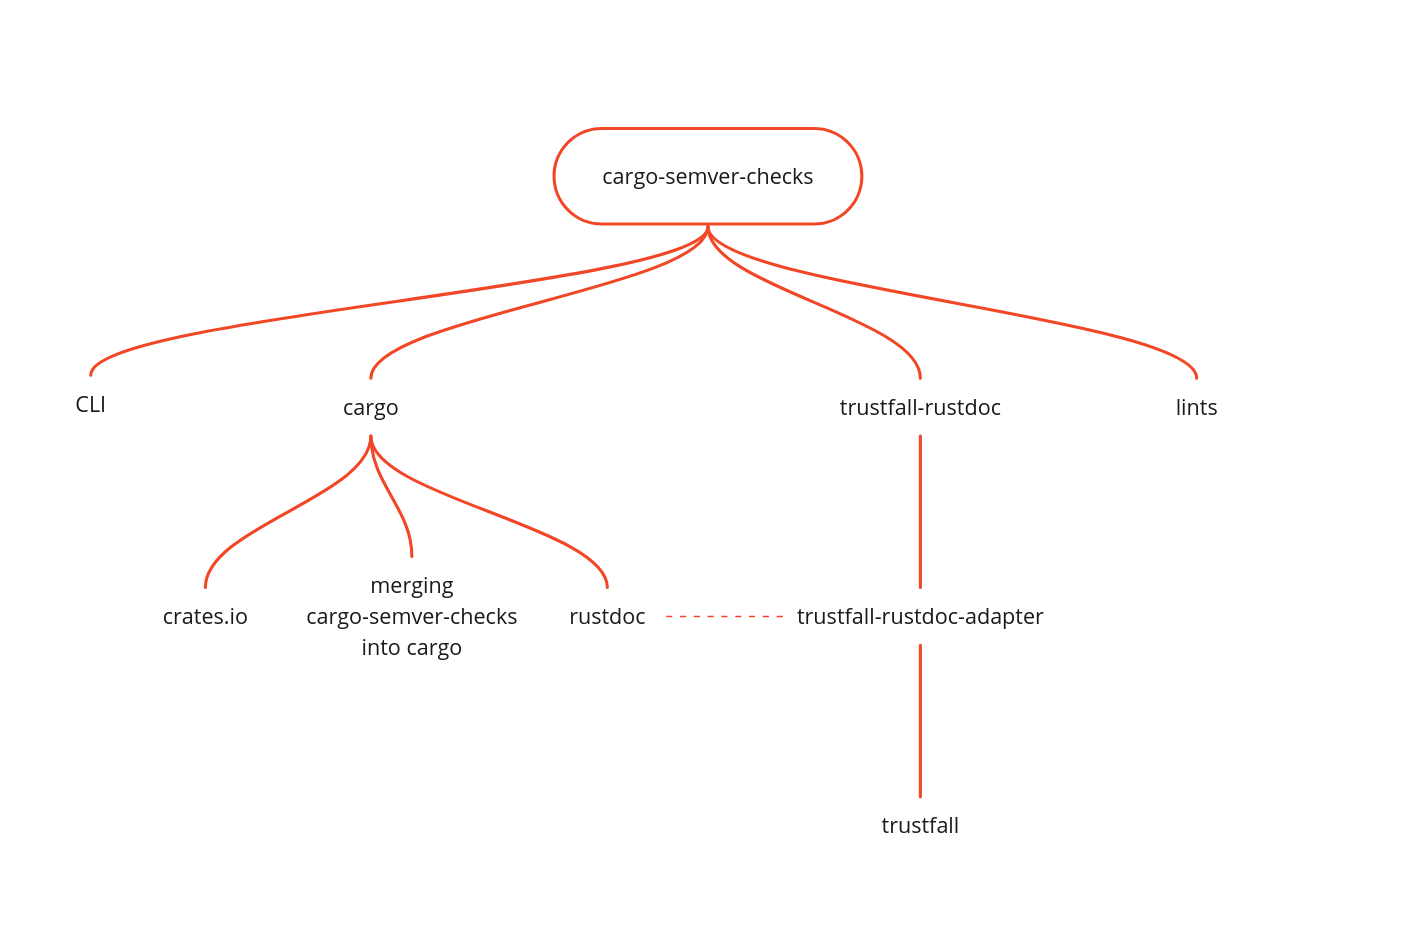
\includegraphics[width=\linewidth]{project-structure-diagram.png}
	\caption{Diagram of the project structure}
\end{figure}

In order to check two versions of a crate for semver violations, the tool needs a consistent method
for generating the data to be compared. This is achieved by using rustdoc (from the official
Rust toolchain) to generate the documentation for Rust projects. However, the documentation itself
often changes its format and thus is not stable nor organized enough to be directly used by
cargo-semver-checks. For this reason, the tool uses Trustfall to access and query the output
received from rustdoc.

Trustfall is a special query engine, designed to query any data source or a combination of data
sources such as APIs, raw files (JSON, CSV, etc.), git version control, webpages and many more.
Its main idea is to represent the data as an organised graph with vertices and edges that the
engine can traverse. To navigate during the search, it follows consecutive filtering rules defined
by the user. In cargo-semver-checks, these rules are contained within \texttt{.ron} files which
are called \texttt{lints} inside the project (more detail in section
\ref{r:section_cargo_semver_checks}).

Despite being the project's core component, new lints are not the only thing we developed. In total
there are four repositories that we have been actively contributing to for the last few months:
\begin{itemize}
	\item \textbf{cargo-semver-checks} -- a CLI (Command Line Interface) tool that runs the lints
		(Trustfall queries),
	\item \textbf{trustfall-rustdoc-adapter} -- implements the Trustfall interface for one specific
		rustdoc version,
	\item \textbf{trustfall-rustdoc} -- allows running Trustfall queries over rustdoc regardless of
		the currently used rustdoc version,
	\item \textbf{cargo-semver-checks-action} -- the tool in form of a GitHub Action that can
	    be added to GitHub repositories.
\end{itemize}

\section{cargo-semver-checks}\label{r:section_cargo_semver_checks}

The goal of cargo-semver-checks is to detect semver violations within Rust crates. Given two
versions of the same crate:
\begin{itemize}
	\item \textbf{baseline} -- the existing version that defines a public API,
	\item \textbf{current} -- the modified version of the baseline that is vulnerable to
		breaking semver,
\end{itemize}
the tool uses Trustfall as a layer of abstraction that remains constant regardless of changes in
the underlying JSON representation format (functions, structs, enums, variants, etc.) To better
visualize this concept, one can imagine a query that asks Trustfall to \say{Find all public Enums
from the baseline version that no longer exist in the current version of the crate}. That kind
of query never makes any statements or assumptions about its data representation or format.

After that, the versions are compared using all of the implemented lints to find the breaking
public API changes. They are the core component of the project and are carefully designed so that
one break can only be reported by one, precise lint. This is especially important because we want
the user to be provided with an extensive, coherent and clear information about the error they
have made.

In cargo-semver-checks, each lint contains a single \texttt{SemverQuery} to execute, consisting of
the following fields:

\begin{itemize}
	\item \texttt{id} -- a short, unique name identifying the lint, most often matching the
		filename that contains the lint,
	\item \texttt{human\_readable\_name} -- a longer, human-readable name,
	\item \texttt{description} -- general information about what is the detected problem,
	\item \texttt{required\_update} -- the minimum version bump needed to avoid breaking semver,
	\item \texttt{reference\_link} -- a link to the official Rust documentation corresponding to
		the issue (when available),
	\item \texttt{query} -- the Trustfall filtering rules responsible for comparing two versions and
		detecting semver violations (described below in more detail),
	\item \texttt{arguments} -- optional, user-defined Trustfall constants for the query,
	\item \texttt{error\_message} -- a longer and more technical information, telling the user
	    about the exact semver violation that occured and what could have caused it,
	\item \texttt{per\_result\_error\_template} -- the name of the item that broke semver and
	    its exact position in the code.
\end{itemize}

\begin{figure}[h]
	\centering
	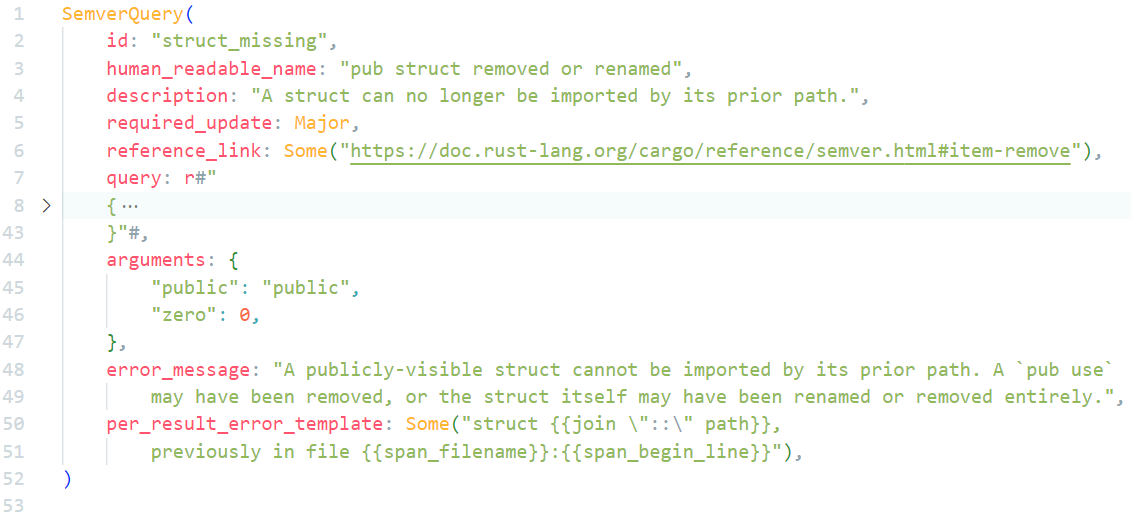
\includegraphics[width=\linewidth]{lint-example.png}
	\caption{The \texttt{enum\_missing} lint (for its entire query, see figure
		\ref{fig:enum_missing_lint_query})}
	\label{fig:enum_missing_lint}
\end{figure}

Each query defines the filtering rules necessary to compare the baseline and current versions of
a crate. They contain elements such as:
\begin{itemize}
	\item \texttt{@tag} -- allows the value to be used elsewhere in the query by
		tagging its name,
	\item \texttt{@filter}, \texttt{@fold}, \texttt{@transform} -- some of the available Trustfall
		directives that modify the sets of items processed by the query,
	\item \texttt{@output} -- specifies which values are returned by the query,
	\item \texttt{@optional} -- edges marked optional are allowed to not exist, in which case
		\texttt{@output} properties within become \texttt{null} instead of causing that result
		to be discarded,
	\item \texttt{... on Enum} -- \texttt{...} narrows that location in the query to the specified
		kind of items (in this case Enums), discarding all results that had other types of data
		in that location
	\item \texttt{\$public}, \texttt{\$zero} -- \texttt{\$} refers to the argument with the same
		name,
	\item \texttt{\%path} -- \texttt{\%} refers to a tagged element with the same name.
\end{itemize}

\begin{figure}[h]
	\centering
	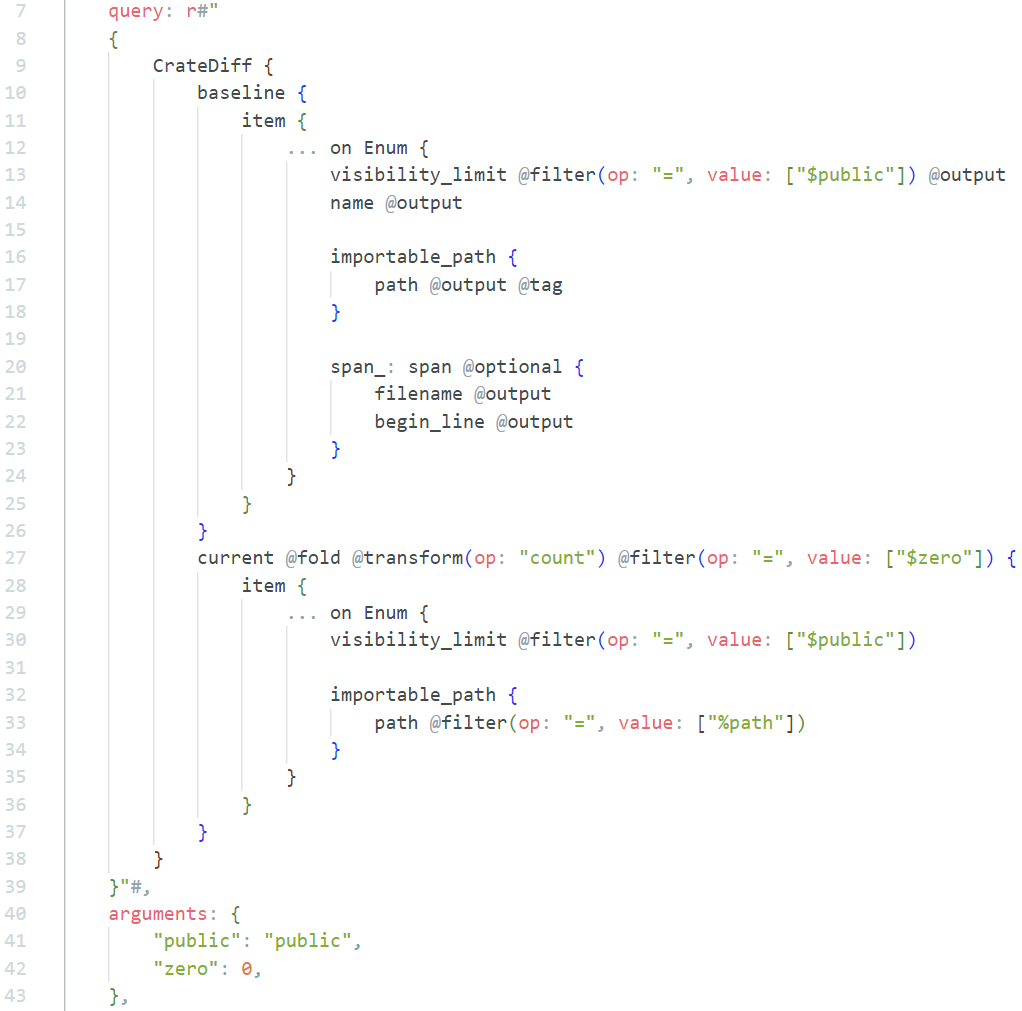
\includegraphics[width=\linewidth]{lint-query-example.png}
	\caption{The \texttt{enum\_missing} lint's query}
	\label{fig:enum_missing_lint_query}
\end{figure}

The query above is part of the lint seen in figure \ref{fig:enum_missing_lint}.
During its execution, Trustfall successively:
\begin{itemize}
	\item collects all of the baseline crate's public Enums, tagging their paths,
	\item collects all of the current crate's public Enums such that their path is present among
		the baseline version's tagged paths,
	\item counts the occurences of the filtered current Enums among the filtered baseline Enums,
	\item filters the current Enums by their resulting count being zero,
	\item returns the Enums that passed the last filtering.
\end{itemize}
Just like that, the query has returned all of the public Enums that were present in the baseline
version of the crate, but got removed in the current version.

\section{trustfall-rustdoc-adapter}\label{r:section_trustfall_rustdoc_adapter}
The output generated by running rustdoc on a crate is a tree and can be in one of the two formats:
\begin{itemize}
	\item HTML -- the default option, formatted with CSS, designed for users to read (however it is
		difficult to parse),
	\item JSON -- convenient for further processing, but practically unreadable to humans due to its
		complex structure and large size of up to a few hundred MB.
\end{itemize}
This makes the JSON format a~natural candidate for running Trustfall queries. However, it still has
to be transformed into a~structure that is understandable for Trustfall, namely a~graph in which
vertices are assigned types and type-dependent properties.

This is where trustfall-rustdoc-adapter comes in. It provides an interface for querying
the rustdoc's output by associating JSON nodes with Trustfall vertices. To achieve this, the adapter
implements the following methods:
\begin{itemize}
	\item \texttt{resolve\_starting\_vertices} -- returns an iterator over the starting vertices of
		the graph (entry points for query executions),
	\item \texttt{resolve\_property} -- resolves the value of a specified vertex' property,
	\item \texttt{resolve\_neighbors} -- finds the neighboring vertices across an edge,
	\item \texttt{resolve\_coercion} -- attempts to coerce a vertex into a more specific type.
\end{itemize}
These are used by the Trustfall engine to execute lint queries written in the Trustfall language.

\section{trustfall-rustdoc}\label{r:section_trustfall_rustdoc}

Rustdoc output format is under constant development and changes between Rust versions.
Since the tool is supposed to be widely used, it is important to ensure that it works with
the recent versions of Rust (and consequently with all recent versions of rustdoc).
Therefore, the trustfall-rustdoc-adapter is developed on several different git branches,
each of them handling a~specific rustdoc version.

The trustfall-rustdoc brings them together in the form of a single tool. Given the path to
the rustdoc JSON output, trustfall-rustdoc loads the file, detects which rustdoc version was used
and chooses the corresponding trustfall-rustdoc-adapter branch to run the Trustfall queries.
This provides a version-independent interface which is used by cargo-semver-checks.

\section{cargo-semver-checks-action}\label{r:section_cargo_semver_checks_action}

Using cargo-semver-checks in a continuous integration workflow consists of three main steps:
setting up the Rust toolchain, installing cargo-semver-checks, and finally -- running it on a~crate.
The aim of the cargo-semver-checks-action is to simplify this process and make it a~single step,
hiding the technical details from the user.

The cargo-semver-checks-action is implemented as a~GitHub Action, which is a~way of creating
a reusable GitHub workflow. It is hosted on a public repository and can be used in continuous
integration by referencing its name and version in the workflow file. Besides being run with default
parameters, the action can be configured by providing optional inputs (such as the name of the crate
to check), which are passed to the CLI of the cargo-semver-checks binary.

The V1 version of the action was implemented as a bash script, which was a~quick, but difficult
to maintain solution, which allowed the action to be run only on Linux hosts. This is why
we implemented the V2 version of the action in a platform-independent way using TypeScript
and Node.js, allowing it to be used on all runners supported by GitHub Actions.
The differences between the V1 and V2 of the action are further discussed in section
\ref{r:section_continuous_integration_improvements}.

%%%%%%%%%%%%%%%%%%%%%%%%%%%%%%%%%%%%%%%
%           Implementation            %
%%%%%%%%%%%%%%%%%%%%%%%%%%%%%%%%%%%%%%%

\chapter{Implementation}\label{r:chapter_implementation}

\section{The lint set expansion}\label{r:section_new_lints}

<Here write a list about the new lints we've written>

\section{Command-line interface improvements}\label{r:section_cli}

<Here write a list about changes that made the command line interface better>

\section{Brand new GitHub Action}\label{r:section_github_action}

<Here write a list about the V2 of the continuous integration>

\section{Test suite}\label{r:section_test_suite}

<Here write a list about the improvements in the testing suite>

\section{Healthier codebase}\label{r:section_healthier_codebase}

TODO:
\begin{itemize}
	\item describe refactors and other changes that made the codebase better
	\item describe other overall changes that prepares the tool to be more successful in the future
	\item describe how the code changed to be more welcoming for next contributors
\end{itemize}

\section{Bugfixes}\label{r:section_bugfixes}

<Here write a list about found and fixed bugs>


% chapter semver-crater
\chapter{Tool's findings in popular crates}\label{r:chapter_results_popular_crates}

\section{Statistics on found true-positives}\label{r:section_results_statistics}

Thanks to cargo-semver-checks, we were able to find numerous true-positives
amongst the one thousand most downloaded Rust crates.
This section presents the results we got and the following one (\ref{r:section_generating_witnesses})
describes how we managed to obtain them.

TODO: calculate Xi constants.

Those crates have X0 total releases (at the time of writing)
that were published after XX-XX-XXXX, X1 of which do not compile anymore with the current version of Rust
and X2 of the remaining ones were yanked.

From the X3 non-yanked releases which we were able to compile,
\textbf{in X4 of them we found one or more semver breaks}.
In total, different lints were triggered X5 times with X6 items reported (one release can trigger multiple lints, each of them reporting multiple items in the sourcecode that broke semver).

For every true-positive we constructed a \texttt{witness} -- a short Rust code
proving that a particular item indeed breaks server.
Each witness can be compiled using one version of a crate
but results in a compilation error for the other version.
Moreover, for each result we have viewed its sourcecode to confirm
that it is part of the public API accessible by the user. Thus, we are confident that each
result is a real true-positive.

The following table shows for each lint in how many releases it was triggered
and how many items in total it has reported:

X7-table

X8-explain-implications

All of the detected true-positives (with their witnesses) can be found in a GitHub repository [X10]
in both human-readable and machine-readable form.
All of the results (both true-positives and false-positives / bugs) are provided
in a human-readable form.

\section{The process of gathering results (semver-crater)}\label{r:section_results_semver_crater}

Because cargo-semver-checks is able to create a rustdoc
from the registry of a particular crate and version,
we thought of running the tool on a large number of existing crates
to find true-positives and bugs (which mostly are false-positives or crashes).
We developed a tool for this purpose and called it \texttt{semver-crater}
(similarly to \texttt{crater} which is used by the Rust team to check
new compilator versions on a large number of crates).

It fetches a list of one thousand crates available on crates.io, sorted by the number of
all-time downloads (thus, they are often the biggest crates and libraries
that strictly adhere to semantic versioning). For each crate,
it then retrieves the available versions which were not yanked
and compares every two adjacent, non-yanked versions and parses the output.
The results (which take several days to generate) are saved to a CSV file.

Unfortunately, cargo-semver-checks is not yet perfect and sometimes produces false-positives
that are to be fixed. However, most of them were caused by one of the two cases:
\begin{itemize}
	\item an item was marked with the \texttt{\#[doc(hidden)]} attribute,
		which hides it from the documentation and thus is not part
		of the public API accessible by the user
		(\texttt{\#[doc(hidden)]} is most often used by macros to hide their generated code
		as it is irrevelant for the user),
	\item an item was moved to another crate and re-exported
		(thus the item is still accessible with the old path,
		but its definition is in another rustdoc making it not visible to cargo-semver-checks).
\end{itemize}
Other false-positives also happened, but they showed up rarely and primarily
were just caused by a bug in the lint query.

Because fixing the two main false-positives turned out to be difficult, we instead shifted our focus
to finding ways for detecting when one of them happened.
We came up with two solutions:
\begin{itemize}
	\item To detect most of the \say{doc hidden} false-positives
		(though not all), we managed to get a list of items that are definitely
		\say{doc hidden} and then ignored such items in the results.
		We were able to create the list by running cargo-semver-checks on one rustdoc
		containing the hidden items and another one without the hidden items,
		parsing the output to know which items were removed.
	\item As a way to know whether a reported item is a false-positive or a true-positive,
		we created a witness (more on that in section \ref{r:witness_generation})
		and ignored all items whose witnesses compile on both baseline and current versions.
\end{itemize}

Those two techniques greatly reduced the number of reports.
To be sure that the remaining items were true-positives,
we manually checked the code (we managed to generate links to the line of code where each item was defined).
Mostly we verified whether an item was indeed a part of the public API
(not below a \say{doc hidden} and not a part of a test module).
With that, we have high confidence that the found items are indeed true-positives.

\section{Generating witnesses}\label{r:section_generating_witnesses}

The fact that a release broke semver can be proven by a \say{witness},
which consists of two small crates:
\begin{itemize}
	\item a \say{baseline} -- a crate which uses the old release as a dependency
		and compiles fine,
	\item a \say{current} -- a crate which uses the new release as a dependency
		and does not compile.
\end{itemize}
Both crates must have exactly the same code (same \texttt{src/lib.rs} file),
but slightly different manifests.
Thus, a witness is made of just three short files -- a source code that uses the item that
broke semver and two manifests that only differ in the \texttt{[dependency]} section
(they have the same crate name as a dependency, but two different versions of it).

The output of each lint in cargo-semver-checks contains a list of importable paths
of items that it was triggered by, which is enough to construct some of the witnesses automatically.

For example, after parsing the output of the \texttt{enum\_variant\_missing} lint,
we got the importable path of the enum and the name of its variant that was removed.
Thanks to that, we were able to write a Rust code with a function that deconstructs the enum
to the given variant. This source code compiles on the baseline, but does not compile
on the current (because the Rust compiler cannot find the variant), thus it is a valid witness.

Using this logic, we wrote a Python script that parses the output of cargo-semver-checks,
generates the witnesses and tries to compile them.
There are three possible outcomes:
\begin{itemize}
	\item the baseline compiles and the current doesn't compile, so it's a correct witness,
	\item both the baseline and current compile, which indicates a false-positive and a bug in cargo-semver-checks,
	\item the baseline does not compile, which means that the witness was constructed incorrectly.
\end{itemize}

We stumbled upon some complications while creating the witnesses for some of the lints.
We had the importable path of an item, but we were missing the information
about generics or traits, which the Rust compiler requires to be in the source code
(e.g. a function could take a generic argument which type needs to be declared when calling the function).
Most cases were solved by writing a script that iterates over the number of generic arguments
and checks whether a witness with some number of generic argument successfully compiles.
The other cases required the generic types to satisfy some traits,
which is much harder to automate or even write manually.
Thus we decided that we would skip checking some of the reports that required using generic types with traits.

For some lints we could choose between simply importing the given item
(e.g. by \texttt{use importable\_path;}) or creating a source code that uses it.
Since just importing the item can be seen as not convincing and not visually appealing (it does not use any item properties,
e.g. it uses the function name but does not call the function itself).
Thus, we decided to generate witnesses with the more convincing technique of writing the more realistic Rust code whenever possible
and used the pure imports as a fallback when it failed to compile.

We had one last difficulty when we tried to create witnesses for the e.g. \texttt{enum\_variant\_added} lint.
To construct a witness for it, one has to exhaustively pattern-match
on all of the given enum's variants. However, the output only contained the name
of the variant that was added rather than a list of all the variants' names.
To retrieve the full list, we wrote a separate
Rust project that uses \texttt{trustfall\_rustdoc} -- given the generated rustdoc of the dependency,
it runs a Trustfall query that finds the enum with matching importable path and returns
all of its variants. Having passed the newly-acquired data to the Python script,
we could then automatically construct its witness.

Some lints were triggered only a couple times, so instead of expanding the Python script's functionality, it was faster to manually write witnesses for them.
There was also the \texttt{struct\_repr\_c\_removed} lint that reported a breaking change.
However, the issue was based on creating an undefined behavior rather than a compilation error,
making it difficult to create a witness.
Thus we decided to make an exception and manually verify whether it was indeed a semver-break.

After all the work, our Python script is able to create the following witness kinds
with the following ways to write them:
\begin{table}[h]
	\centering
	% adjust the fractions here so that it looks nice (MUST sum up to 1)
	\begin{tabular}{| p{.5\linewidth} | p{.5\linewidth} |}
		\hline
			\multicolumn{1}{|Sc|}{\textbf{lint}} &
			\multicolumn{1}{Sc|}{\textbf{witness description}} \\
		\hline
			\begin{tabular}[c]{@{}l@{}}
				\texttt{enum\_missing} \\
				\texttt{struct\_missing}
			\end{tabular} &
			\multicolumn{1}{Sl|}{\parbox{.5\linewidth}{
				a (possibly generic) function that takes the item as an argument
			}} \\
		\hline
			\begin{tabular}[c]{@{}l@{}}
				\texttt{trait\_missing}
			\end{tabular} &
			\multicolumn{1}{Sl|}{\parbox{.5\linewidth}{
				a generic function (with possibly multiple generic arguments) that takes
				a generic argument satisfying the trait
			}} \\
		\hline
			\begin{tabular}[c]{@{}l@{}}
				\texttt{function\_missing} \\
				\texttt{method\_missing} \\
				\texttt{function\_parameter\_count\_changed} \\
				\texttt{method\_parameter\_count\_changed}
			\end{tabular} &
			\multicolumn{1}{Sl|}{\parbox{.5\linewidth}{
				executing the function with an adequate number of \texttt{todo!()} arguments.
				This technique creates valid witnesses, even though it gives a warning that
				such statements are unreachable (it is still possible to replace
				the \texttt{todo!()} argument with manually constructed ones, but it's not needed
				to show a semver break)
			}} \\
		\hline
			\begin{tabular}[c]{@{}l@{}}
				TODO \texttt{trait\_implementation\_removed}
			\end{tabular} &
			\multicolumn{1}{Sl|}{\parbox{.5\linewidth}{
				a helper function that takes a generic argument satisfying the given trait
				and a (possibly generic) function that takes the item and passes it to
				the helper function
			}} \\
		\hline
			\begin{tabular}[c]{@{}l@{}}
				\texttt{enum\_variant\_missing}
			\end{tabular} &
			\multicolumn{1}{Sl|}{\parbox{.5\linewidth}{
				deconstructing the enum with an \texttt{if} to the given variant
			}} \\
		\hline
			\begin{tabular}[c]{@{}l@{}}
				\texttt{enum\_variant\_added} \\
				\texttt{enum\_marked\_non\_exhaustive} \\
				\texttt{struct\_field\_added}
			\end{tabular} &
			\multicolumn{1}{Sl|}{\parbox{.5\linewidth}{
				pattern-matching on all of the item's variants or fields
			}} \\
		\hline
	\end{tabular}
\end{table}

%%%%%%%%%%%%%%%%%%%%%%%%%%%%%%%%%%%%%%%
%                Team                 %
%%%%%%%%%%%%%%%%%%%%%%%%%%%%%%%%%%%%%%%
\chapter{Team}\label{r:chapter_team}

\section{Used methodology}\label{r:section_used_methodology}

The project's functionalities and goals can be split into independent improvements, hence our
contributions were mostly composed of multiple smaller changes. The usual workflow of writing
code was as follows:
\begin{enumerate}
	\item discussing with our mentor (who is also the project maintainer) about which improvements
		have the highest priority,
	\item individually picking a few tasks based on our preferences,
	\item implementing those tasks (and sometimes also thinking about the design of the change)
		and creating Pull Requests on the project's GitHub repositories,
	\item going through an extensive review process with our mentor (as there are often other
		contributors in the project besides us, the code's readability is a strong focus point
		in the project),
	\item getting the Pull Request merged by our mentor and releasing (usually a few days later)
		a new version of the binary to the registry.
\end{enumerate}

There were some exceptions to this workflow:
\begin{itemize}
	\item at the beginning, we split into two pairs and our mentor gave each of us introductory
		tasks to work on together and familiarize with different aspects of the existing code,
	\item to speedup the process of merging the Pull Requests, we sometimes reviewed each others'
		code before passing it to our mentor,
	\item when a user reported a bug, we often looked into the problem and searched for a temporary
		fix of the bug as soon as possible,
	\item when we encountered bugs or thought of possible additional improvements in the tool's
		functionality, we created an appropriate Issue on the GitHub repository.
\end{itemize}

Additionally, we held weekly meetings with the four of us to discuss the progress and future
contributions (we did not need to have regular meeting with our mentor, because we had constant
and immediate contact with him through chat).

\section{Responsibilities}\label{r:section_responsibilities}

\begin{itemize}
	\item Tomasz \cite{responsibilities-tomasz}:
		\begin{itemize}
			\item Reported a bug with an incorrect path to the generated rustdoc when passing
				a manifest path in the CLI.
			\item Changed how the manifest of the baseline is built and added selecting all
				features to baseline's manifest, which resolved an issue reported by a user of
				the tool where the current and baseline's rustdoc was generated with different
				features, which resulted in false-positives.
			\item Reported a bug where the tests failed on the newest version of the compiler
				and implemented a fix.
			\item Renamed directories with queries and tests, thanks to which the structure of
				the project is now clear, more intuitive and updated \texttt{CONTRIBUTING.md}.
			\item Replaced code duplication with a Rust macro and made adding new lints easier.
			\item Improved the tests, which sped up the process of adding new lints.
				More precisely:
				\begin{itemize}
					\item splitted each test into separate pairs of crates (that are baseline
						and current crates for the tool),
					\item made it so that the tool runs each lint on all testing crates
						(which has detected multiple new false-positives),
					\item massively improved the readability and ease of adding new tests and lints,
					\item improved the error messages when the test output didn't match.
				\end{itemize}
			\item Made a change in the tests that runs the tool on crates that did not change
				to detect possible false-positives.
			\item Commited changes suggested by a new version of the Rust formatter.
			\item Found and fixed a bug where the printed baseline version was incorrect.
			\item Added a new type of integration tests, which locally checks how the tool behaves
				with given commandline arguments, and implemented a test that checks whether
				a recent bug (where the lint files were not present in the binary) was fixed.
			\item Diagnosed a problem where the tests stopped working, fixed the adapter after
				a new rustdoc version which stopped exporting inlined items of external crates
				and created an issue for strengthening back a lint that was affected
				by those changes.
			\item Reported a problem where the user could be confused by the lack of detailed
				information in the help messages of the tool.
			\item Reported a problem where the output of the tool on the \texttt{bevy-audio} crate
				seemed like it was producing a false positive.
			\item Reported a bug where a lint's output was duplicated on the
				\texttt{bevy-render} crate.
			\item Added a feature to disable the usage of the vendored \texttt{OpenSSL} because
				there were problems with it amongst users having the Arch Linux desktop distribution.
			\item Changed the way in which the rustdoc of a crate is generated -- instead of
				directly running the rustdoc command on a local copy of the crate, it is now ran
				on a temporary placeholder project, which just has the checked crate as
				a dependency. It solves a bug encountered by a user where running the tool updates
				the \texttt{Cargo.lock} file, and allows to easily specify the set of
				crate's features to run the rustdoc command on.
				% The change was done by moving and splitting existing functions into smaller ones,
				% switching the baseline rustdoc generation to using the new placeholder project,
				% changing functions' arguments for better readability, renaming files for the same
				% reason, chosing variable names that fit more nicely with the current code
				% and finally switching to the new rustdoc generation logic.
			\item Reported a bug where the tool failed to work when generating rustdoc of a crate
				that only has yanked releases.
			\item Reported a bug where the tool prints some internal data while cheching
				the \texttt{clap} crate.
			\item Found and fixed a bug where the CI job wrongly checked the exit code in one
				of the integration tests.
			\item Added a lint in the CI for checking the rustdoc of the project.
			\item Fixed a broken link which the users saw in the tool's output.
			\item Reported a false-positive which was related to re-exporting types, values
				and macros with the same names.
			\item Fixed a user-encountered bug where implicit features due to target-specific
				optional dependencies were not added in the current version.
			\item Fixed a user-reported bug where the rustdoc command's output wasn't showing up
				with colors.
			\item Diagnosed a user-encountered compilation error which happened because of changes
				in one of the tool's dependencies.
			\item Took part in the development of the library based on the existing tool's code.
		\end{itemize}

	\item Michał \cite{responsibilities-michal}:
		\begin{itemize}
			\item Added a new type of tests in the CI -- a regression test that is checking
				the tool against a specific version of a user's crate, to be certain that now
				the tool works and has no false-positives on it.
			\item Added a test that checks whether a field in the lints is correctly initialized.
			\item Added an integration test in the CI for specifying the package name.
			\item Made a new release workflow in the CI that triggers when publishing a new version
				of the tool and uploads the new binaries to GitHub releases, thanks to which
				the GitHub Actions (both provided by us and written by users for their own purposes)
				that were using the tool can now just download the binary (instead of compiling it),
				which makes the CI job much faster.
			\item Added a new lint (trustfall query, test crates, tests) to detect tuple structs
				that changed to plain structs.
			\item Added a new lint (trustfall query, test crates, tests) that checks whether
				a trait becomes or stops being unsafe and added an \texttt{unsafe} type property
				to \texttt{Trait} in the schema and the adapter.
			\item Added a \texttt{fields} edge to the \texttt{Variant} interface in the schema
				and the adapter.
		\end{itemize}

	\item Tomasz and Michał:
		\begin{itemize}
			\item Added a new lint (trustfall query, test crates, tests) to detect field removals
				from a struct variant in enums and added a field in the adapter for the lint.
			\item Added a new lint (trustfall query, test crates, tests) to detect when function
				and method parameter count changes and added the retrieval of function parameter
				names in the adapter.
			\item Fixed a bug where the rustdoc of the current and the baseline crates
				were overwriting each other, which has been reported by a user.
		\end{itemize}

	\item Mieszko \cite{responsibilities-mieszko}:
		\begin{itemize}
			\item Reported an incorrect behavior of the CLI which was choosing the latest release
				from the registry as a baseline version even when it had been yanked.
				Introduced a fix and created a set of unit tests for choosing the baseline crate.
			\item Reported a problem in release \texttt{v0.18.2} where the CLI was not looking for
				the baseline in the registry as it was supposed to do.
			\item Reported a bug where the precompiled tool crashed on Windows machines.
				Added a CI job that checks for similar issues.
			\item Developed a new version of \texttt{cargo-semver-checks-action}, which consisted of:
			\begin{itemize}
				\item creating a test repository \cite{responsibilities-mieszko-action-tests}
					and using it to add a CI workflow that tests the basic functionalities of
					the action, then further developing the CI tests to cover all options added in
					the new version,
				\item making use of \texttt{cargo-semver-checks} built-in baseline choosing logic,
					which fixed the user-reported issue,
				\item adding support for running the action on Windows- and MacOs-based runners,
				\item introducing input \texttt{manifest-path}, as requested by a user,
				\item introducing input \texttt{verbose}, as requested by a user,
				\item using pre-build binaries to speed up the action, as requested by a user,
				\item rewriting the documentation of the action.
			\end{itemize}
		\end{itemize}

	\item Bartosz \cite{responsibilities-bartosz}:
		\begin{itemize}
			% \item \emph{SCRIBE!} \\
			% This scribe was like no other, \\
			% His notes could make a person shudder, \\
			% Each word he wrote, a work of art, \\
			% A skill that set him far apart. \\

			% Meetings became a grand event, \\
			% When his pen and paper were present, \\
			% Colleagues vied for his attention, \\
			% To ensure their words got a mention. \\

			% For this scribe's notes were legendary, \\
			% Capturing every detail, quite extraordinary, \\
			% No meeting was complete without his touch, \\
			% A true master of the notetaking clutch. \\

			\item Added several new lints (trustfall queries, test crates, tests) to detect
				when different items have been marked with the \texttt{must\_use} attribute.
				Writing separate lints for individual items allowed to provide more detailed
				messages for the user, improved the code structure by creating smaller,
				more specialized files and made the final review process easier. The items that
				undergo those checks are:
				\begin{itemize}
					\item enums,
					\item structs,
					\item traits,
					\item functions,
					\item methods,
					\item inherent methods (reported only when one was both moved to a public trait
						and marked with the attribute).
				\end{itemize}
		\end{itemize}

	\item Mieszko and Bartosz:
		\begin{itemize}
			\item Added a new lint (trustfall query, test crates, tests) to detect when
				an exhaustive public enum has the \texttt{non\_exhaustive} attribute added.
			\item Designed and implemented a new adapter schema for handling attributes.
				Updated all lints that check attributes to use the new schema, as well as added
				multiple new test cases to the queries.
		\end{itemize}
\end{itemize}


%%%%%%%%%%%%%%%%%%%%%%%%%%%%%%%%%%%%%%%
%             Conclusion              %
%%%%%%%%%%%%%%%%%%%%%%%%%%%%%%%%%%%%%%%
\chapter{Conclusion}\label{r:chapter_conclusion}

\section{The significance of our contributions}\label{r:section_significance_of_contributions}

TODO:
\begin{itemize}
	\item write a conclusion
\end{itemize}

\section{Rust community's positive response to the tool}\label{r:section_community_response}

TODO:
\begin{itemize}
	\item show how the number of downloads has changed
	\item show how the number of stars on GitHub has changed
	\item describe how our work might have impacted those results
	\item show the comments of users on GitHub.
		As one of the examples, give the maintainer of a big
		library that created an issue \say{Make continuous integration runs faster}
		and after learning about one of our PRs to make the continuous integration faster,
		he was so excited that he wrote a comment with a tip in our PR.
		Search also for other such examples in the PRs and issues.
	\item list the maintainers of big libraries that started using the tool during our development
\end{itemize}

%%%%%%%%%%%%%%%%%%%%%%%%%%%%%%%%%%%%%%%
%            Bibliography             %
%%%%%%%%%%%%%%%%%%%%%%%%%%%%%%%%%%%%%%%

\appendix

\begin{thebibliography}{99}
\addcontentsline{toc}{chapter}{Bibliography}

%%% template

% \bibitem[Bea65]{beaman} Juliusz Beaman, \textit{Morbidity of the Jolly
%     function}, Mathematica Absurdica, 117 (1965) 338--9.


%%% section 1.1 links

% \bibitem{Rust-1} Rust Team,
% 	\textit{Rust Programming Language} (2023) \\
% 	\url{https://www.rust-lang.org/}

% \bibitem{Rust-2} Wikipedia,
% 	\textit{Rust (programming language)} (2023) \\
% 	\url{https://en.wikipedia.org/wiki/Rust_(programming_language)/}

\bibitem{survey} Stack Overflow,
	\textit{Annual Developer Survey} (2022) \\
	\url{https://insights.stackoverflow.com/survey/}

% \bibitem{Rust-for-Linux} Wikipedia,
% 	\textit{Rust for Linux} (2023) \\
% 	\url{https://en.wikipedia.org/wiki/Rust_for_Linux/}


%%% section 1.2 links

% \bibitem{Cargo} Rust Team,
% 	\textit{The Cargo Book} (2023) \\
% 	\url{https://doc.rust-lang.org/cargo/index.html/}

% \bibitem{python-pip} Wikipedia,
% 	\textit{Python pip} (2023) \\
% 	\url{https://en.wikipedia.org/wiki/Pip_(package_manager)}

% \bibitem{Cargo-vs-pip} William Manley,
% 	\textit{Pip and Cargo are not the same} (2022) \\
% 	\url{https://doc.rust-lang.org/cargo/index.html/}


%%% section 1.3 links

% \bibitem{Semantic-Versioning} semver.org,
% 	\textit{Semantic Versioning 2.0.0} (2022) \\
% 	\url{https://semver.org/}

% \bibitem{fearless-cargo-update} Predrag Gruevski,
%     \textit{Towards fearless cargo update} (2022) \\
%     \url{https://predr.ag/blog/toward-fearless-cargo-update/}


%%% section 1.4 links

% \bibitem{Abstract-Syntax-Tree} Wikipedia,
% 	\textit{Abstract syntax tree} (2023) \\
% 	\url{https://en.wikipedia.org/wiki/Abstract_syntax_tree/}


%%% section 2.1 links

\bibitem{issue-libp2p} GitHub,
	\textit{rust-libp2p -- Pull Request \#3312} (2023) \\
	\url{https://github.com/libp2p/rust-libp2p/pull/3312}


%%% section 2.2 links

\bibitem{issue-compiling-fails} GitHub,
	\textit{cargo-semver-checks -- Issue \#317} (2023) \\
	\url{https://github.com/obi1kenobi/cargo-semver-checks/issues/317}


%%% section 2.3 links

\bibitem{pyo3-issue} GitHub,
    \textit{PyO3 -- Issue \#285} (2018) \\
    \url{https://github.com/PyO3/pyo3/issues/285}

\bibitem{clap-issue} GitHub,
    \textit{clap -- Issue \#3876} (2022) \\
    \url{https://github.com/clap-rs/clap/issues/3876}

\bibitem{block-buffer-issue} GitHub,
    \textit{RustCrypto -- Issue \#22} (2023) \\
    \url{https://github.com/RustCrypto/utils/issues/22}

\bibitem{paper} Hao Li, Filpe R Cogo, Cor-Paul Bezemer, \\
    \textit{An Empirical Study of Yanked Releases in the Rust Package Registry} (2022) \\
	\url{https://arxiv.org/pdf/2201.11821.pdf}


%%% section 2.4 links

\bibitem{elm-lang} Evan Czaplicki,
    \textit{Elm Programming Language} (2021) \\
    \url{https://elm-lang.org/}


%%% section 3.2 links

\bibitem{issue-merge-cargo} GitHub,
	\textit{cargo-semver-checks -- Issue \#61} (2023) \\
	\url{https://github.com/obi1kenobi/cargo-semver-checks/issues/61}

\bibitem{issue-cli-interface} GitHub,
	\textit{cargo-semver-checks -- Issue \#86} (2023) \\
	\url{https://github.com/obi1kenobi/cargo-semver-checks/issues/86}


%%% section 4.1 links

% \bibitem{rustdoc-theory} Rust Team,
% 	\textit{The rustdoc book} (2023) \\
% 	\url{https://doc.rust-lang.org/rustdoc/what-is-rustdoc.html}

% \bibitem{trustfall} GitHub,
% 	\textit{Trustfall -- Query (Almost) Everything} (2023) \\
% 	\url{https://github.com/obi1kenobi/trustfall}


%%% section 4.2 links

% \bibitem{cargo-semver-checks} GitHub,
% 	\textit{cargo-semver-checks} (2023) \\
% 	\url{https://github.com/obi1kenobi/cargo-semver-checks}


%%% section 7.2 links

\bibitem{responsibilities-tomasz} GitHub,
	\textit{Contributions authored by Tomasz} (2023) \\
	\url{https://github.com/search?o=desc&q=org%3Aobi1kenobi+author%3Atonowak&s=updated&type=Issues}

\bibitem{responsibilities-michal} GitHub,
	\textit{Contributions authored by Michał} (2023) \\
	\url{https://github.com/search?o=desc&q=org%3Aobi1kenobi+author%3Astaniewzki&s=updated&type=Issues}

\bibitem{responsibilities-mieszko} GitHub,
	\textit{Contributions authored by Mieszko} (2023) \\
	\url{https://github.com/search?o=desc&q=org%3Aobi1kenobi+author%3Amgr0dzicki&s=updated&type=Issues}

\bibitem{responsibilities-mieszko-action-tests} GitHub,
	\textit{mgr0dzicki/cargo-semver-action-ref-slice} (2023) \\
	\url{https://github.com/mgr0dzicki/cargo-semver-action-ref-slice}

\bibitem{responsibilities-bartosz} GitHub,
	\textit{Contributions authored by Bartosz} (2023) \\
	\url{https://github.com/search?o=desc&q=org%3Aobi1kenobi+author%3ASmolSir&s=updated&type=Issues}

\end{thebibliography}


%%%%%%%%%%%%%%%%%%%%%%%%%%%%%%%%%%%%%%%
%             Attachments             %
%%%%%%%%%%%%%%%%%%%%%%%%%%%%%%%%%%%%%%%

\chapter*{Attachments}
\addcontentsline{toc}{chapter}{Attachments}

\section*{Source code structure}

<Here describe the project structure of the included CD>


\section*{Tests}

<Here describe the tests (and possibly how to run them) of the included CD>

\end{document}


%%% Local Variables:
%%% mode: latex
%%% TeX-master: t
%%% coding: latin-2
%%% End:
